\documentclass[10pt,a4paper]{article}
\usepackage[margin=2cm]{geometry}
\usepackage{amsmath,amssymb}
\usepackage{booktabs}
\usepackage{graphicx}
\usepackage{float}
\usepackage{xcolor}
\usepackage{fontspec}
\usepackage{hyperref}
\usepackage{enumitem}
\usepackage{fancyvrb}
\setlist{nosep,leftmargin=*}
\setmainfont{texgyrepagella}[Extension=.otf,UprightFont=*-regular,BoldFont=*-bold,ItalicFont=*-italic,BoldItalicFont=*-bolditalic]
\setmonofont{DejaVuSansMono}[Extension=.ttf,BoldFont=*-Bold,Scale=0.82]
\hypersetup{colorlinks=true,linkcolor=blue!50!black,urlcolor=blue!50!black}
\newcommand{\RtwoKone}{77.3}\newcommand{\RtwoKfive}{77.3}\newcommand{\RtwoKfiveB}{86.7}
\newcommand{\RtwoValid}{96.6\%}\newcommand{\RtwoN}{2{,}703}

\title{\vspace{-1.2cm}A Neuro-Symbolic Entailment Reasoner:\\ Natural Language $\rightarrow$ Logic $\rightarrow$ Classical Reasoning}
\author{Nikhil Jha \quad (Roll Number: R25CS0001)}
\date{}

\begin{document}
\maketitle
\vspace{-1cm}

\section{Overview}
The system decides whether a natural-language statement is entailed by a natural-language knowledge base. A \emph{router} sends each (context, statement) pair to the cheapest route that can represent it soundly:

\begin{center}
\small
\resizebox{\linewidth}{!}{%
\begin{tabular}{@{}llll@{}}
\toprule
Route & NL $\rightarrow$ representation & Representation & Classical reasoning \\
\midrule
\texttt{causal} & deterministic causal grammar & structural causal model (SCM) & abduction / action / prediction \\
\texttt{horn}   & deterministic RuleTaker grammar & Horn clauses with negation & tabled backward chaining (CWA) \\
\texttt{hybrid} & grammar + LLM for unparsed sentences & Horn clauses with negation & tabled backward chaining (CWA) \\
\texttt{fol}    & fine-tuned LLM semantic parser ($k$ samples) & first-order logic & resolution refutation + vote \\
\bottomrule
\end{tabular}}
\end{center}

\noindent\textbf{Use of the LLM.} The LLM is used only as a semantic parser: it outputs formulas, never a label, and its output is never read as an answer. Every True/False decision is made by the classical engines described in Section~\ref{sec:algo}, which are implemented from scratch in Python (no external prover or logic library).

\section{Representation}
\label{sec:repr}
\paragraph{Horn literals.} A literal is a Python tuple \texttt{(pred, arg$_1$, \dots)}; negation is encoded in the predicate name (\texttt{\~{}p}), so the fact base is a hash set with $O(1)$ membership. Variables are strings starting with \texttt{?}. Adjectives become unary predicates and relations become binary predicates over entity constants:
\begin{center}\small
\begin{tabular}{@{}ll@{}}
\emph{The bald eagle does not chase the cat.} & \texttt{(\~{}chase, bald\_eagle, cat)} \\
\emph{If someone is round and not red then they chase the lion.} & $\mathit{round}(x)\wedge\neg\mathit{red}(x)\rightarrow \mathit{chase}(x,\mathit{lion})$ \\
\emph{Kind, furry things are quiet.} & $\mathit{kind}(x)\wedge\mathit{furry}(x)\rightarrow\mathit{quiet}(x)$
\end{tabular}
\end{center}

\paragraph{First-order logic.} An AST with \texttt{atom}, $\neg$, $\wedge$, $\vee$, $\rightarrow$, $\leftrightarrow$, $\oplus$, $\forall$, $\exists$; terms are constants, variables or Skolem functions. Clauses are frozensets of signed literals.

\paragraph{Structural causal model.} Boolean equations $V := \mathrm{op}(\ell_1,\dots,\ell_n) \oplus \mathit{neg}$ with $\mathrm{op}\in\{\wedge,\vee\}$ over a DAG, exogenous priors $P(U{=}1)$ (from ``$X\sim\mathrm{Bern}(p)$''), and observations.

\section{From natural language to the representation}
\paragraph{RuleTaker grammar.} A regular grammar over sentence shapes, not vocabulary: entities are matched by shape (capitalised name, ``the'' + up to three nouns, or a quantifier pronoun), verbs are lemmatised (\emph{chases}$\rightarrow$\emph{chase}), and elliptical conjuncts (\emph{``is round and red''}) inherit the previous subject. Unseen names, adjectives and verbs therefore parse unchanged. Coverage on all public RuleTaker splits (including the \texttt{NatLang} configurations) is 100\%.

\paragraph{Causal grammar.} Splits ``\emph{A and B together cause not C, D causes E and F}'' into equations, detects observations, priors and the three question forms (``\emph{would Y occur if not X instead of X}'', joint and nested interventions).

\paragraph{LLM semantic parser.} Qwen2.5-14B-Instruct (bf16) with a LoRA adapter ($r{=}32$) served by vLLM on two A30 GPUs. The model outputs one formula per premise plus the conclusion; our own FOL parser validates syntax and predicate arity, and an invalid output is sent back once with the parser's error message (repair loop). For each problem, $k{=}3$ translations are sampled (the first greedily). In the \texttt{hybrid} route only the sentences the grammar cannot parse are translated; definite formulas $\forall x\,(\bigwedge_i \ell_i \rightarrow \ell)$ are mapped to Horn rules with the grammar's naming (CamelCase $\rightarrow$ snake case, verbs lemmatised). Generic nouns that the grammar reads as the unrestricted domain (\emph{person}, \emph{thing}, \emph{someone}) are dropped from rule bodies when the theory never states them, so \emph{``every person that is round is rough''} becomes $\mathit{round}(x)\rightarrow\mathit{rough}(x)$ in both parsers.

\paragraph{Solver-verified self-training.} FOLIO's training split ships gold FOL, but running our prover on it showed that only \textbf{583 of 1{,}001} annotations reproduce their own gold label (typos such as \texttt{Studen}, inconsistent predicates such as \texttt{Writtenby}/\texttt{Write}, free variables). We therefore train only on translations that our prover \emph{verifies}: a pair is kept if proving the translated conclusion from the translated premises yields the gold label. Candidates come from the gold annotations and from $k{=}5$ model samples on FOLIO-train. Because a disconnected translation is trivially ``Uncertain'', a model translation is additionally required to use only conclusion predicates that occur in the premises. Round 1 trains on 1{,}885 verified pairs (583 gold + 1{,}302 model samples from 14B and 32B); round 2 resamples the training set with the round-1 model and retrains on \RtwoN{} pairs. FOLIO validation is never used for training; it is used once per round to choose the adapter.

\section{Reasoning algorithms}
\label{sec:algo}
\paragraph{Forward chaining (closed world).} RuleTaker's labels follow the closed-world assumption with negation as failure (Table~\ref{tab:rt}). Rules may test $\neg p$ while $p$ is derived by other rules, and evaluating such programs by \emph{predicate-level} stratification is too coarse: on RuleTaker it produces 98.7\%, because cycles through negation exist between predicates (\texttt{need}$\rightarrow$\texttt{young}$\rightarrow$\texttt{visit}$\leftarrow\neg$\texttt{need}) even though the ground atoms are acyclic. We instead compute the \textbf{well-founded model} with the alternating fixpoint: $\Gamma(S)$ is the least model in which $\neg p$ holds iff $p\notin S$; iterating $T\leftarrow\Gamma(\Gamma(T))$ from $T=\emptyset$ converges to the true atoms, which equals the perfect model for every program that is stratified at the ground level. Each fixpoint is computed by rule matching against a predicate-indexed fact base (most-bound literal first); every derived fact records its rule and premises for traces.

\paragraph{Backward chaining (default engine).} SLD resolution with negation as failure: only rules whose head unifies with the goal are tried; positive literals are solved before negated ones so that negation is tested on ground atoms. A ground goal already on the ancestor stack fails (loop check). Completed goals are tabled and the table is shared across all questions about the same context; a failure is tabled only if no loop cut occurred beneath it, since such a failure may succeed via another branch. Backward chaining agrees with the well-founded forward model on all 227{,}783 public RuleTaker questions and is $1.6$--$5\times$ faster (Figure~\ref{fig:fcbc}), so it is the default engine for the \texttt{horn} route.

\paragraph{Resolution refutation.} $\mathit{KB}\models\varphi$ is decided by deriving $\square$ from $\mathit{KB}\wedge\neg\varphi$: elimination of $\rightarrow,\leftrightarrow,\oplus$; NNF; standardisation apart; Skolemisation; CNF. Two classical techniques keep CNF polynomial: \textbf{Tseitin naming} replaces non-literal operands of $\oplus/\leftrightarrow$ by fresh predicates with definitional axioms (a 14-way $\oplus$ chain in FOLIO otherwise expands to $2^{13}$ copies), and distribution of $\vee$ over $\wedge$ above 32 clauses names one side instead. The search is a given-clause loop with \textbf{set of support} (only clauses descending from $\neg\varphi$ are selected), \textbf{best-first} selection by clause weight (UCS on symbol count), binary resolution with most-general unification (occurs check), binary \textbf{factoring}, deletion of tautologies, variants (clauses are canonicalised up to variable renaming) and subsumed clauses, and a term-depth bound. Equality axioms (reflexivity, symmetry, transitivity, substitution for each predicate argument) are added when ``='' occurs. The three-way verdict (used for analysis) is True if $\mathit{KB}\models\varphi$, False if $\mathit{KB}\models\neg\varphi$, else Uncertain. The task's label is binary, so the router runs only the refutation of $\mathit{KB}\wedge\neg\varphi$ per sample and predicts True iff a strict majority of the $k$ samples are entailed; for $k{=}3$ this equals the plurality of three-way verdicts with ties towards ``not entailed'', and it halves reasoning time because the expensive $\mathit{KB}\models\neg\varphi$ attempts on Uncertain problems are skipped. Independent problems are refuted in parallel (process pool).

\paragraph{Counterfactual inference.} Pearl's three steps, solved exactly by enumerating the exogenous worlds: (1) \emph{abduction}: keep worlds consistent with the observations; an observed variable whose equation disagrees with the observation is explained by an exogenous leak/inhibitor term (prior $10^{-3}$), which then persists into the counterfactual world; (2) \emph{action}: replace the equations of intervened variables; (3) \emph{prediction}: evaluate the query variable in topological order (DFS). The answer with the larger posterior mass wins.

\section{Experiments on the public datasets}
\label{sec:exp}
All timings are wall-clock on one CPU core of the login node (reasoning) and on NVIDIA A30 GPUs (LLM translation).

\begin{table}[H]
\centering\small
\caption{RuleTaker (grammar + backward chaining). Dev was used for development; test was evaluated once.}
\label{tab:rt}
\begin{tabular}{@{}lrrrrrrrrr@{}}
\toprule
 & d0 & d1 & d2 & d3 & d3ext & d5 & NatLang & d3ext-NL & \textbf{all} \\
\midrule
dev questions & 8{,}718 & 8{,}870 & 8{,}906 & 8{,}896 & 11{,}587 & 9{,}486 & 3{,}899 & 15{,}510 & 75{,}872 \\
open world (explicit negation) & 77.9 & 74.3 & 72.9 & 73.6 & 73.9 & 75.3 & 75.6 & 74.3 & 74.6 \\
closed world, predicate strata & 100 & 100 & 99.4 & 97.8 & 98.3 & 96.5 & 100 & 98.7 & 98.7 \\
\textbf{closed world, well-founded} & \textbf{100} & \textbf{100} & \textbf{100} & \textbf{100} & \textbf{100} & \textbf{100} & \textbf{100} & \textbf{100} & \textbf{100} \\
\midrule
test (151{,}911 questions) & 100 & 100 & 100 & 100 & 100 & 100 & 100 & 100 & \textbf{100} \\
\bottomrule
\end{tabular}
\end{table}

\begin{figure}[H]
\centering
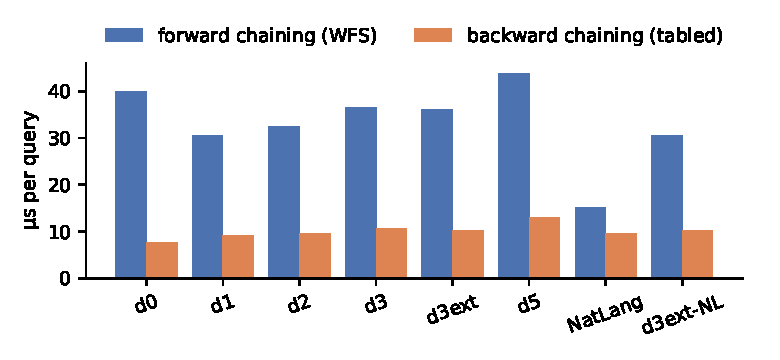
\includegraphics[width=0.62\linewidth]{fig_fc_bc.pdf}
\caption{Reasoning time per RuleTaker query (dev). Backward chaining with tabling explores only rules relevant to the question and shares its table across all questions of a context.}
\label{fig:fcbc}
\end{figure}

\paragraph{Grammar vs.\ LLM translation on templated text.} Sending 115 questions of the paraphrased RuleTaker configuration (d3ext-NL) through the LLM $\rightarrow$ FOL $\rightarrow$ resolution route instead of the grammar gives 82.6\% ($k{=}1$) and 85.2\% ($k{=}5$), against 100\% for the grammar, at roughly $10^5\times$ the cost. Deterministic parsing is used whenever it applies.

\begin{table}[H]
\centering\small
\caption{CounterBench (1{,}200 questions, 0.2\,s in total).}
\label{tab:cb}
\begin{tabular}{@{}lrrrrrr@{}}
\toprule
 & basic & conditional & joint & nested & backdoor & \textbf{all} \\
\midrule
accuracy (\%) & 100.0 & 92.0 & 96.0 & 96.0 & 87.5 & \textbf{94.6} \\
\bottomrule
\end{tabular}
\end{table}
\noindent All 65 errors come from 13 graph structures, each repeated with 5 name sets. At least 50 of them contradict every observation semantics we tested (ignore, hold fixed, XOR noise, leak/inhibitor). For example, after $do(V_3{=}0)$ the only cause of $V_4$ is false, yet the gold label says $V_4$ occurs. We keep the principled semantics instead of fitting these labels.

\begin{table}[H]
\centering\small
\caption{FOLIO validation (203 problems; 72 True / 62 False / 69 Uncertain). Binary = entailed vs.\ not entailed. LLM time is for all $203\times5$ samples.}
\label{tab:folio}
\begin{tabular}{@{}lccccr@{}}
\toprule
Translator (all followed by our resolution prover) & valid FOL & 3-way $k{=}1$ & 3-way $k{=}5$ & binary $k{=}5$ & LLM time \\
\midrule
Gold FOL annotations (no LLM) & 100\% & \multicolumn{2}{c}{73.9} & 85.7 & -- \\
Qwen2.5-14B-AWQ, 3-shot & 94.8\% & 61.1 & 61.6 & 78.3 & 256\,s \\
Qwen2.5-32B-AWQ, 3-shot (2$\times$A30) & 96.1\% & 70.4 & 74.4 & 86.7 & 337\,s \\
14B + LoRA, round 1 (zero-shot) & 97.1\% & 78.8 & 79.3 & 88.7 & 441\,s \\
14B + LoRA, round 2 (zero-shot) & \RtwoValid & \RtwoKone & \RtwoKfive & \RtwoKfiveB & 449\,s \\
\bottomrule
\end{tabular}
\end{table}

\noindent\textbf{Prover vs.\ annotation quality.} On the 134 decisive validation problems, the prover run on the gold FOL proves 81, \emph{saturates} on 41 (the gold formulas do not entail the gold label: annotation errors) and reaches its limit on 12. It never answers True when the label is False. Solver-verified fine-tuning lets a 14B model exceed both the gold annotations (+5.4 three-way) and a 32B few-shot model (+4.9); voting over samples helps the few-shot models more than the fine-tuned one, whose samples are already consistent.

\noindent\textbf{A second self-training round does not help.} Round 2 adds 818 verified pairs, mostly sampled from the round-1 model itself, and scores 77.3\% (vs.\ 79.3\% at $k{=}5$; a difference of about four problems). Two factors are confounded: fewer epochs (2 vs.\ 3) and self-reinforcement, since label agreement is weak evidence for ``Uncertain'' problems and the round-1 model's own consistent errors are re-learned. We keep the round-1 adapter with $k{=}3$ (79.8\% three-way, 89.2\% binary).

\paragraph{End-to-end system.} Table~\ref{tab:e2e} runs the complete router (final configuration: round-1 adapter, $k{=}3$). The paraphrase set is a robustness test we built from RuleTaker dev: in 150 contexts, one or two rules are rewritten into meaning-preserving forms the grammar does not cover (\emph{``Anyone who is cold and not quiet is also young''}, \emph{``Every person that is big is cold''}), so gold labels stay valid. Without the LLM these contexts cannot be parsed (42.4\%, all answered ``not entailed''); with the \texttt{hybrid} route all 623 hybrid questions are answered correctly. The remaining 23 questions come from short contexts in which fewer than 60\% of the sentences parse, so the router treats them as open-world text (\texttt{fol} route, 17/23 correct); we do not lower this threshold because FOLIO contexts also reach 60--67\% grammar coverage.

\begin{table}[H]
\centering\small
\caption{Complete system. LLM time is uncached generation on 2$\times$A30 (model load: 70\,s, once); reasoning time on CPU. The FOLIO samples are an independent run, so the number differs slightly from Table~\ref{tab:folio} (88.7--89.2\%).}
\label{tab:e2e}
\begin{tabular}{@{}lrrlrr@{}}
\toprule
Dataset & questions & accuracy & routes & LLM & reasoning \\
\midrule
RuleTaker dev & 75{,}872 & 100.00 & horn & -- & 2.0\,s \\
RuleTaker test & 151{,}911 & 100.00 & horn & -- & 4.0\,s \\
CounterBench & 1{,}200 & 94.58 & causal & -- & 0.3\,s \\
FOLIO validation (binary) & 203 & 87.68 & fol & 250\,s & 6.0\,s \\
RuleTaker paraphrased (ours) & 646 & 99.07 & hybrid 623 / fol 23 & 72\,s & 0.2\,s \\
\bottomrule
\end{tabular}
\end{table}

\section{Reasoning traces}
\begin{Verbatim}[fontsize=\footnotesize,frame=single,label={RuleTaker, backward chaining with negation as failure}]
Context: Dave is red. If something is red and not furry then it is white.   Query: Dave is white.
white(dave)   [by red(?x) ∧ ¬furry(?x) → white(?x)]
  red(dave)   [fact]
  ¬furry(dave)   [negation as failure]                                         -> True
\end{Verbatim}
\begin{Verbatim}[fontsize=\footnotesize,frame=single,label={Assignment example, proof tree}]
successful(bob)   [by smart(?x) ∧ kind(?x) → successful(?x)]
  smart(bob)   [by young(?x) → smart(?x)]
    young(bob)   [fact]
  kind(bob)   [fact]                                                             -> True
\end{Verbatim}
\begin{Verbatim}[fontsize=\footnotesize,frame=single,label={CounterBench, counterfactual}]
Ziklo causes Blaf, Blaf causes Trune, Trune causes Vork, Vork causes Lumbo.
Q: Would Lumbo occur if not Ziklo instead of Ziklo?
abduction: Ziklo=1 (factual), no leaks | action: do(Ziklo=0) | prediction: Blaf=Trune=Vork=Lumbo=0 -> False
\end{Verbatim}
\begin{Verbatim}[fontsize=\footnotesize,frame=single,label={Resolution refutation}]
KB: ∀x (Dog(x) → Animal(x)),  Dog(rex)            goal: Animal(rex)
¬Animal(rex)  +  ¬Dog(x) ∨ Animal(x)  ⇒  ¬Dog(rex)
¬Dog(rex)     +  Dog(rex)             ⇒  □                                     -> entailed
\end{Verbatim}

\section{Efficiency and limitations}
All 228{,}983 public RuleTaker and CounterBench queries are answered in about 6\,s on one CPU core without any LLM; the LLM is loaded only if some input cannot be parsed deterministically, and its translations are cached. For FOLIO, the binary one-direction vote and parallel refutation reduce reasoning time from 53\,s to 6\,s with identical accuracy; translation (about 1.2\,s per problem for $k{=}3$) dominates. Limitations: the grammar covers RuleTaker's sentence shapes, so paraphrased Horn text needs the LLM (hybrid route), and short, heavily paraphrased contexts are treated as open-world text; resolution is bounded (1\,s and 6{,}000 clauses per refutation in the router), so a few true entailments are reported as not entailed; the CounterBench semantics is principled but does not reproduce 65 gold labels.

\end{document}
